\begin{comment}


The followed informations introduce the results of two different tests 
using POV-Ray.

In the first test, Fig. \ref{fig:imgpapercerta}, 
the algorithm makes the tracking of an object through 14 images in sequence with 
a horizontal displacement to the camera.

\begin{figure}[H]
\centering
  \subfloat[]{\label{fig:imgpapercertaa} 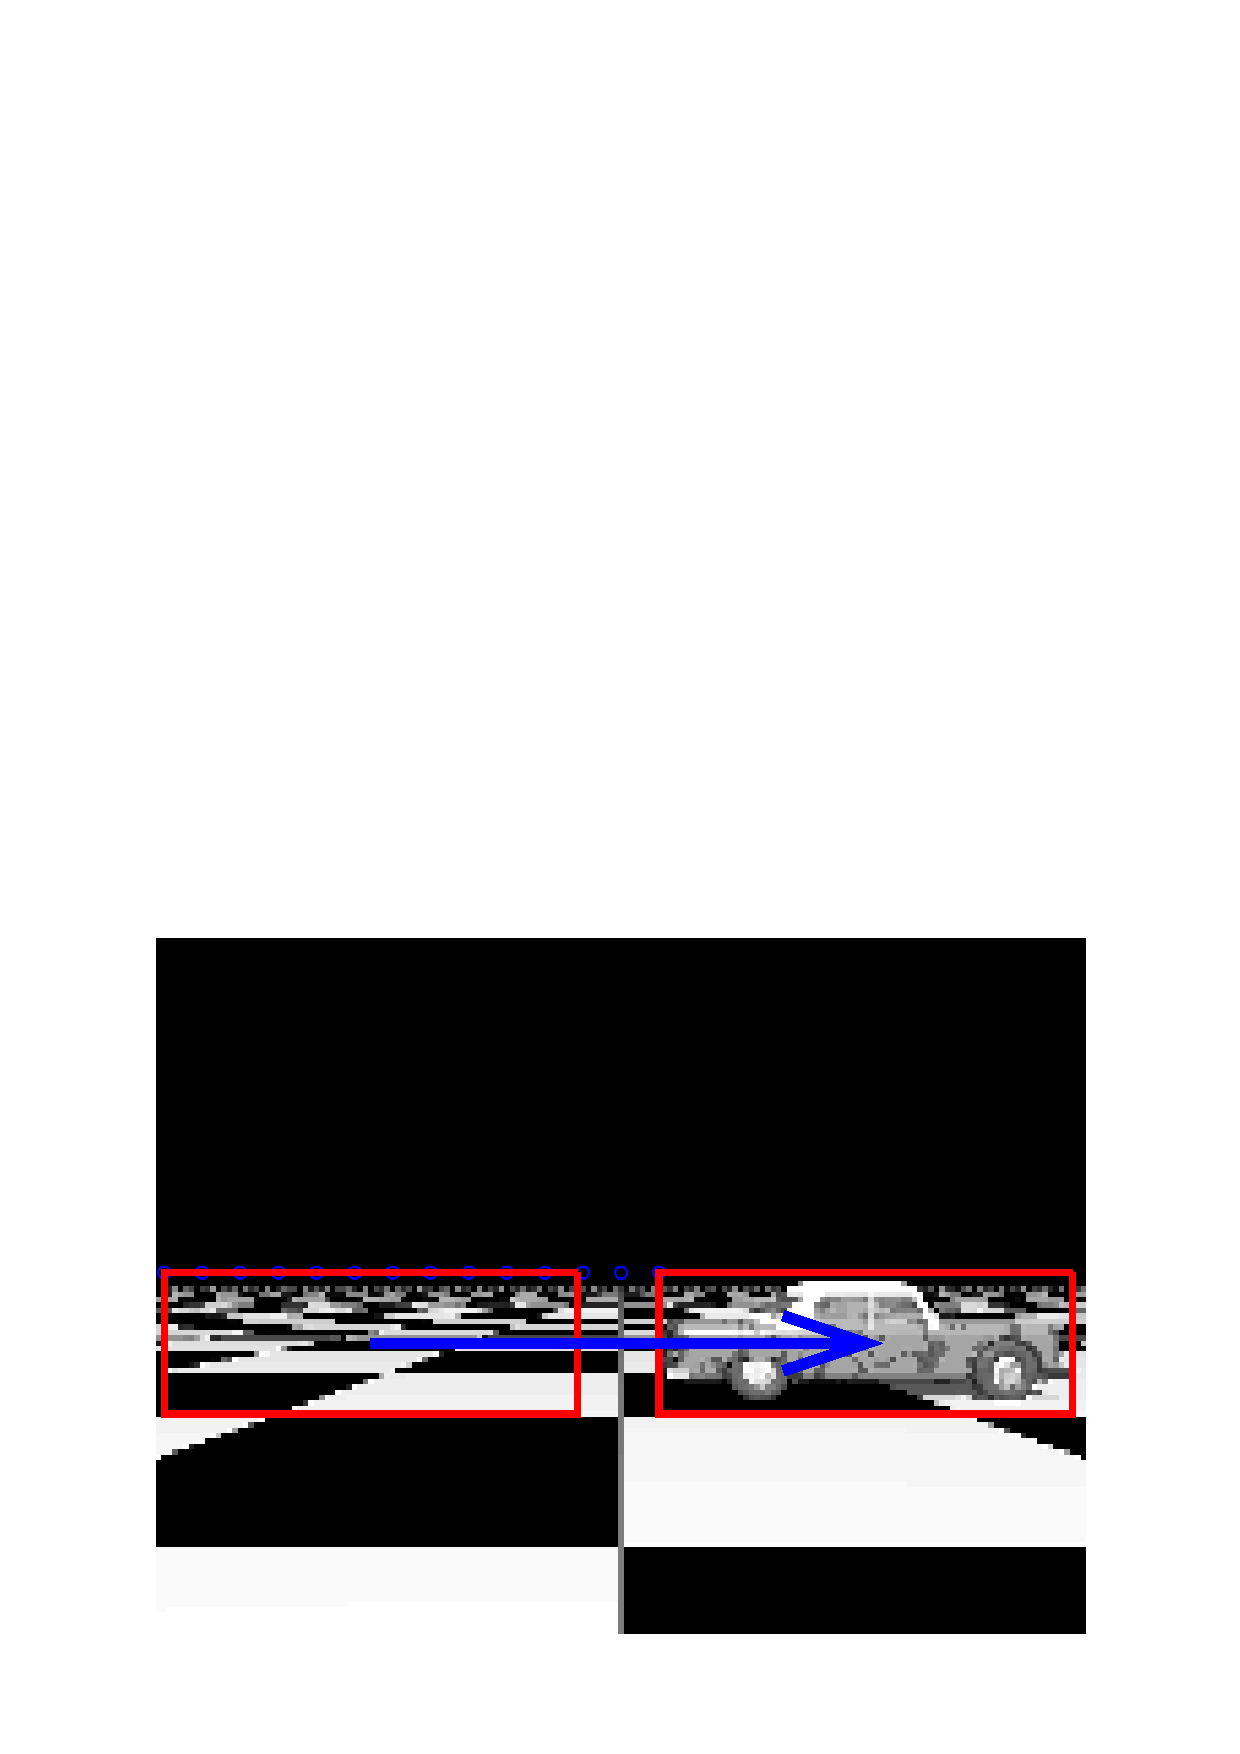
\includegraphics[width=.48\columnwidth]{images/results_2D.png}}
  \subfloat[]{\label{fig:imgpapercertab} 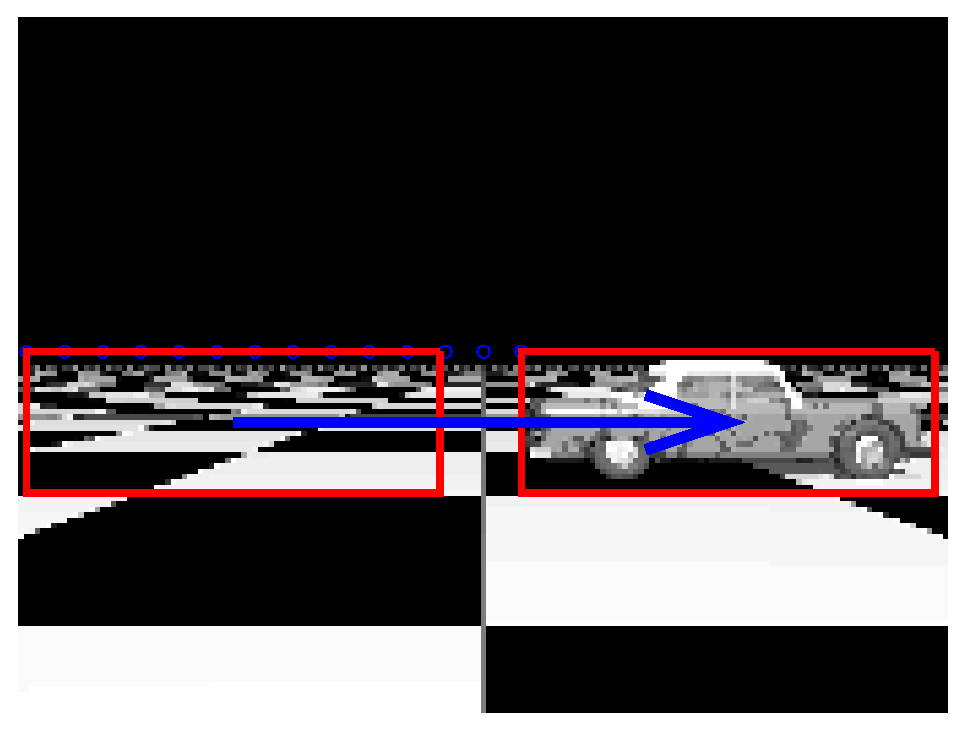
\includegraphics[width=.48\columnwidth]{images/results_2D.eps}}
  \caption{The image in (a) represents the target in its initial position 
   and the image (b) shows the vehicle in its final position.}
  \label{fig:imgpapercerta}
\end{figure}

The initial position of target is in the image (a) and the final position in (b), 
where a vector (in blue) illustrates the resulting trace.
We can observe that there is a small bend in the image 
and it generates a slight change of object perspective. 
The update of the $ROI$ is frequently done, which involves seeing a slight change in area.
The difference between the initial and final values of the departure factor may 
be considered constant, and the value is 1. It means that image doesn't approach to the camera
%as shown in Fig. \ref{fig:res_graph1}.

%\begin{figure}[H]
%\centering
%\includegraphics[width=0.8\columnwidth]{images/results2D_graph.eps}
%\caption{Departure factor for each frame in the test 1.}
%\label{fig:res_graph1}
%\end{figure}

%Fig. \ref{fig:res_graph1v} shows 
The value of the velocity of departure factor is $d_0=1$ and $\Delta t=1$. 
It demonstrates that the variation
of the departure factor is 0 when compared with 1. 
It has departure factor (velocity) of $0$. Target is at same distance 
during 14 frames in relation camera.
.
%\begin{figure}[H]
%\centering
%\includegraphics[width=0.8\columnwidth]{images/results2D_graphv.eps}
%\caption{Velocity of departure factor for each frame in the test 1.}
%\label{fig:res_graph1v}
%\end{figure}

In test 1, we can observed the movement in axis X and rotation of target, the last one causes change of ROI more frequent
because CCP generates a value below of threshold defined in Fig. \ref{fig:newroicri}.
The high changes of ROI for rotation of target can be showed by bubbles in the superior part of ROI in Fig. 
\ref{fig:imgpapercerta} (b).

\end{comment}

%%%%%%%%%%%%%%%%%%%%%%%%%%%%%%%%%%%%%%%%%%portugues%%%%%%%%%%%%%%%%%%%%%%%%%%%%%%%%%%%%%%%%%%%%%%%


Os resultados a seguir foram obtidos em testes usando o simulador POV-Ray.
No primeiro teste, o algoritmo foi submetido a uma sequência de 14 imagens 
com apenas um objeto de interesse que estava em movimento horizontal em relação a câmera, 
como mostrado na Figura \ref{fig:imgpapercerta}.
\begin{figure}[H]
\centering
  \subfloat[]{\label{fig:imgpapercertaa} 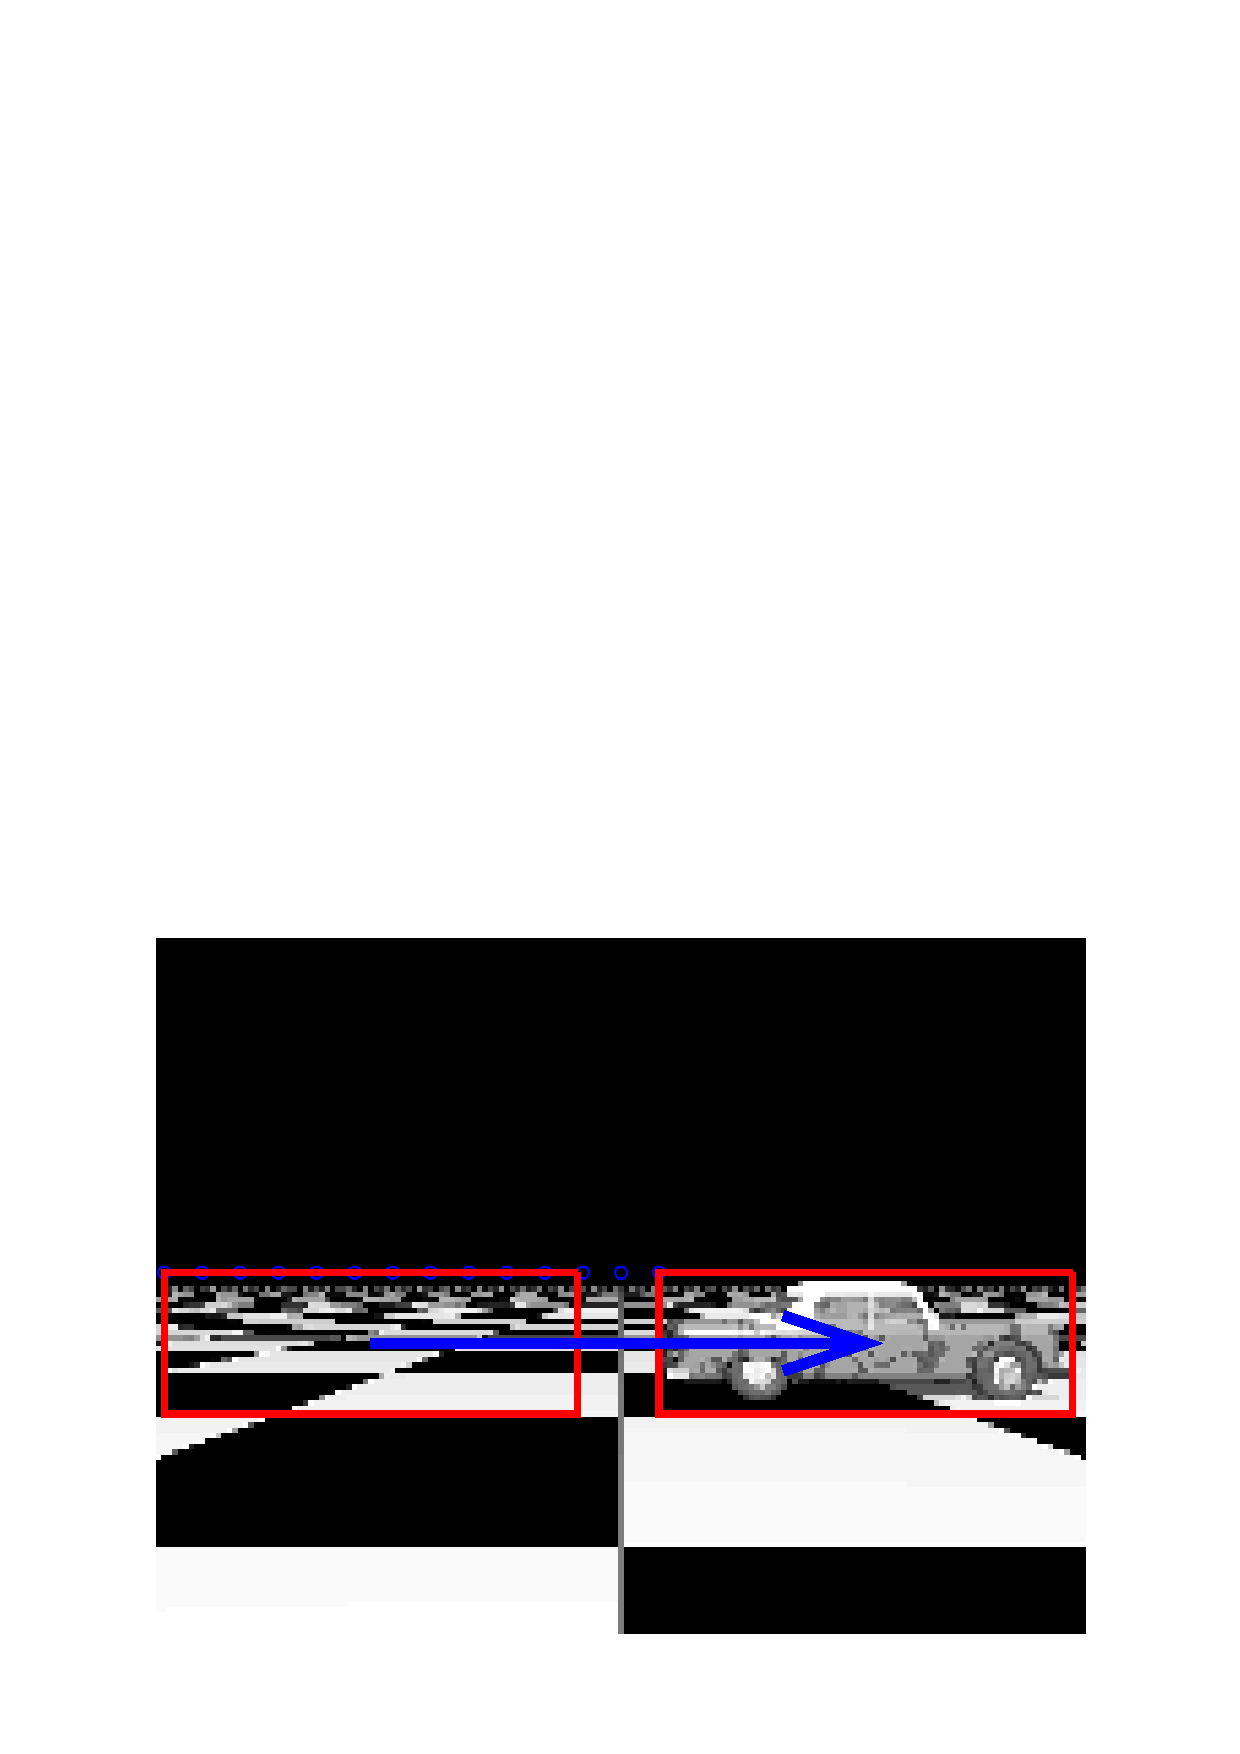
\includegraphics[width=.48\columnwidth]{images/results_2D.png}}
  \subfloat[]{\label{fig:imgpapercertab} 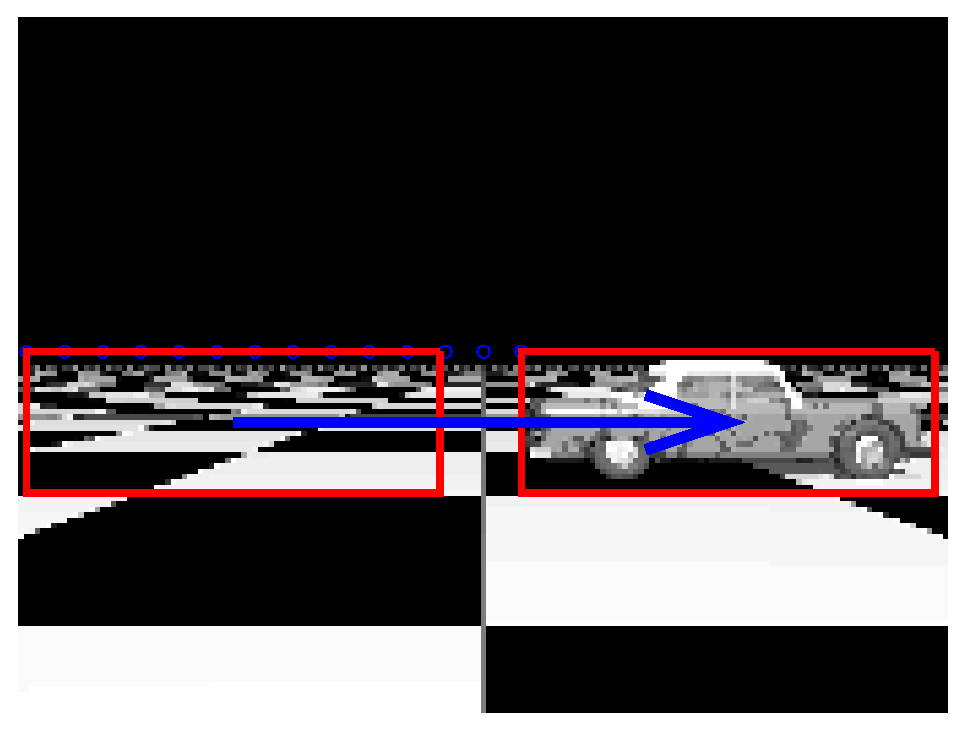
\includegraphics[width=.48\columnwidth]{images/results_2D.eps}}
  \caption{A imagem (a) apresenta o objeto de interesse  em sua posição inicial  
   e a imagem (b) mostra o mesmo objeto na sua posição final.}
  \label{fig:imgpapercerta}
\end{figure}

A posiçao inicial do objeto de interesse está na Figura \ref{fig:imgpapercerta}(a), 
e a  posição final do mesmo na Figura \ref{fig:imgpapercerta}(b). 
O vetor em azul é o resultado do rastreamento do objeto, ligando a posição inicial com a final.
Nota-se uma pequena curvatura na imagem ocasionada por uma mudança
na perspectiva do objeto, resultando em uma mudança frequente da $ROI$.
A diferença entre o valor inicial e final do fator de aproximação $\beta$ (relativo a $d_0$) observado é  constante
e tem valor aproximado  igual a 1, pois o objeto não se aproxima da câmera, realiza apenas um deslocamento horizontal.
Neste teste, a velocidade do fator de aproximação é zero, pois não há aproximação e nem
afastamento do objeto em relação a câmera, sendo $\beta d_0 \approx 1$ e $\Delta t=1$.
Observa-se uma modificação frequente no $ROI$ e isso ocorre pois as imagens 
tem uma correlação menor (valor de $CCP$ menor que $0,8$), como apresentado na Figura \ref{fig:newroicri}.
